\def\r{3em}
\def\angle{10}
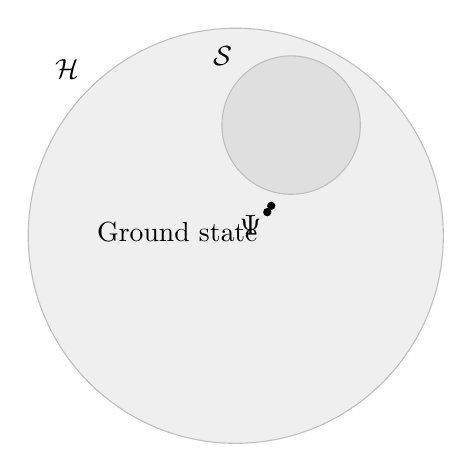
\begin{tikzpicture} 
	
	\node[
		name=H,
		circle,
		draw=lightgray,
		text=black,
		fill=lightgray!25,
		minimum size=15em
	] 
		(H) at (0,0) {};
		
	\node[anchor=south east] at (H.north west)
		{$\mathcal{H}$};

	\node[
		name=S,
		circle,
		draw=lightgray,
		text=black,
		fill=lightgray!50,
		minimum size=5em
	] 
		(S) at (2em,4em) {};
		
	\node[anchor=south east] at (S.north west)
		{$\mathcal{S}$};
		
	\fill 
		(0.4,0.3) circle (1.5pt)
			node[anchor=north east]
				{Ground state};

	\fill 
	(0.45,0.38) circle (1.5pt)
		node[anchor=north east]
			{$\ket{\Psi}$};

\end{tikzpicture}
